\chapter{SISTEM \textit{ELECTRIC BIKE-SHARING} DI KOTA YOGYAKARTA}

Dalam bab ini akan dibahas pembentukan model sistem \textit{electric bike-sharing} mulai dari asumi-asumsi, notasi, fungsi tujuan, serta kendala. Permasalahan utama dalam masalah optimalisasi ini yaitu memaksimalkan keuntungan berdasarkan pemilihan stasiun peminjaman, trip yang diterima, dan jumlah sepeda listrik yang perlu dibeli. Permasalahan ini akan dimodelkan menggunakan model \textit{two-stage stochastic} dengan kendala pada tahap pertama terfokus pada perencanaan jangka panjang yaitu lokasi stasiun dan kapasistas sistem (sepeda dan pengisian daya) dan kendala pada tahap kedua berkaitan dengan operasi harian sistem. Model \textit{two-stage stochastic} yang disusun ini akan diselesaikan dengan algortima \textit{fire-hawk optimizer}.

Dalam studi kasus ini, lokasi sistem \textit{electric bike-sharing} yang digunakan dalam simulasi berlokasi di Yogyakarta dengan Tugu Yogyakarta sebagai titik tengah sistem. Selain itu skenario yang digunakan meliputi hari kerja (\textit{weekdays}), Sabtu (\textit{Saturday}), dan Minggu (\textit{Sunday}), dengan probabilitas skenario Minggu yang paling besar, diikuti Sabtu, kemudian hari kerja memiliki probabilitas paling kecil. 

\section{Pemodelan Sistem \textit{Electric Bike-Sharing}}
Sistem \textit{electric bike-sharing} muncul sebagai solusi transportasi perkotaan yang menjanjikan, menawarkan mobilitas yang fleksibel dan ramah lingkungan. Untuk merancang dan mengoperasikan sistem ini secara efisien memerlukan pendekatan canggih untuk mengatasi berbagai tantangan, termasuk ketidakpastian permintaan, manajemen pengisian daya, dan optimalisasi jaringan (\mycitet{brandstatter2017determining}).

\subsection{Kompleksitas Sistem \textit{Electric Bike-Sharing}}
Sistem \textit{electric bike-sharing} memiliki beberapa karakteristik unik yang membuatnya lebih kompleks dibandingkan sistem \textit{bike-sharing} tradisional:
\begin{enumerate}
    \item \textbf{Manajemen Baterai}\\ Sistem menggunakan metode pengisian daya langsung (\textit{direct charging}) yang mana sepeda listrik diisi dayanya saat terparkir di stasiun, bukan menggunakan sistem penukaran baterai (\textit{battery swapping}).
    \item \textbf{Variabilitas Permintaan}\\ Pola permintaan sangat bervariasi tergantung pada waktu, cuaca, dan acara khusus, memerlukan pendekatan yang fleksibel.
    \item \textbf{Optimalisasi Jaringan}\\ Penempatan stasiun yang optimal harus mempertimbangkan tidak hanya aksesibilitas tetapi juga ketersediaan infrastruktur pengisian daya.
    \item \textbf{Keseimbangan Sistem}\\ Menjaga keseimbangan antara ketersediaan sepeda dan slot pengisian di seluruh jaringan merupakan tantangan yang berkelanjutan.
\end{enumerate}

\subsection{Pendekatan Pemodelan Stokastik Dua Tahap}
Untuk mengatasi kompleksitas ini, diadopsi pendekatan pemodelan stokastik dua tahap. Pendekatan ini digunakan karena cocok untuk digunakan dalam pengaplikasian permasalahan transportasi yang melibatkan ketidakpastian.

\begin{enumerate}
    \item \textbf{Tahap Pertama}
    
    Dalam tahap pertama ini keputusan yang diambil  melibatkan perencanaan strategis jangka panjang yaitu terkait lokasi stasiun dan kapasitas sistem.
    \begin{enumerate}
        \item [\textbf{a.}] \textbf{Lokasi Stasiun}\\ Penentuan stasiun pengisian dibangun dengan mempertimbangkan beberapa faktor seperti kepadatan populasi, dan infrastruktur yang ada.
        \item [\textbf{b.}] \textbf{Kapasitas Sistem}\\ Penentuan jumlah sepeda listrik yang akan dibeli dan kapasitas pengisian di setiap stasiun.
    \end{enumerate}
Keputusan ini dibuat sebelum mempertimbangkan permintaan, berdasarkan proyeksi dan analisis skenario. Kemudian setelah ketidakpastian diketahui, dapat ditentukan keputusan pada tahap kedua.

 \item \textbf{Tahap Kedua}
 
    Dalam tahap kedua keputusan yang diambil berkaitan dengan operasi harian sistem.
    \begin{enumerate}
    \item [\textbf{a.}] \textbf{Alokasi Sepeda}\\ Penentuan distribusi sepeda di seluruh jaringan untuk memenuhi permintaan.
    \item [\textbf{b.}] \textbf{Penerimaan Trip}\\ Pengambilan trip mana yang akan diterima berdasarkan ketersediaan sepeda dan status pengisian daya.
    \item [\textbf{c.}] \textbf{Manajemen Pengisian Daya}\\ 
    Manajemen pengisian daya mengikuti beberapa protokol, setiap sepeda yang kembali dari trip langsung masuk ke mode pengisian daya, sepeda dalam status pengisian tidak tersedia untuk trip baru, dan waktu pengisian bergantung pada sisa kapasitas baterai saat kembali.
    \end{enumerate}

Keputusan ini dibuat secara \textit{real-time} atau \textit{near-real-time} setelah permintaan aktual diketahui. Keputusan pada tahap pertama dan tahap kedua diintegrasikan berdasarkan komponen utama model.
\end{enumerate}


\subsection{Komponen Utama Model}
Model yang dikembangkan mengintegrasikan beberapa komponen penting meliputi:
\begin{enumerate}
    \item \textbf{Representasi Jaringan}\\ Dalam hal ini digunakan graf berbobot untuk merepresentasikan jaringan stasiun dan rute perjalanan.
    \item \textbf{Pemodelan Permintaan}\\ Pendekatan berbasis skenario akan diadopsi untuk menangkap variabilitas permintaan.
    \item \textbf{Dinamika Sistem}\\ Graf lokasi \textit{time-expanded} digunakan untuk memodelkan pergerakan sepeda, status pengisian daya, dan alokasi trip dengan setiap titik merepresentasikan kombinasi lokasi stasiun dan waktu diskrit, sementara \textit{arc} menggambarkan aktivitas seperti pengisian daya (\textit{waiting arc}), perjalanan (\textit{travel ar}c), serta penempatan awal dan akhir sepeda.
    \item \textbf{Kendala Anggaran dan Operasional}\\ Batasan finansial dan teknis akan dipertimbangkan dalam pengambilan keputusan.
\end{enumerate}

\subsection{Struktur Model}
Model diformulasikan dengan program linear bilangan bulat stokastik, struktur ini dapat mengintegrasikan komponen-komponen di atas untuk masalah optimisasi sistem \textit{electric bike-sharing}.
\begin{enumerate}
    \item \textbf{Fungsi Tujuan}\\ Tujuan adalah memaksimalkan ekspektasi keuntungan, menyeimbangkan pendapatan dari trip yang diterima dengan biaya operasional dan investasi.
    \item \textbf{Kendala Tahap Pertama}\\ Kendala meliputi kendala anggaran, kapasitas sistem, dan lokasi stasiun.
    \item \textbf{Kendala Tahap Kedua}\\ Kendala mencakup keseimbangan alur sepeda bergerak, manajemen pengisian daya, dan pemenuhan permintaan.
    \item \textbf{Variabel Keputusan}\\ Kombinasi variabel biner dan kontinu untuk merepresentasikan keputusan diskrit (seperti pembangunan stasiun) dan kontinu (seperti alokasi sepeda).
\end{enumerate}

\section{Asumsi dan Notasi}

Selanjutnya, dijelaskan mengenai asumsi-asumsi model, yang sebagian besar berdasarkan \mycite{brandstatter2017determining} dengan beberapa modifikasi.
\begin{enumerate}
    \item \textbf{Perkiraan Permintaan}\\ Diasumsikan tersedia perkiraan permintaan pelanggan untuk berbagai skenario (hari kerja) dengan probabilitas terkait. Setiap skenario mencakup set perkiraan trip yang mempertimbangkan aspek spasial dan temporal permintaan.
    \item \textbf{Informasi Trip}\\ Setiap trip memiliki informasi lengkap tentang lokasi asal, tujuan, waktu mulai, dan waktu selesai. Informasi ini memungkinkan estimasi konsumsi baterai dan kontribusi profit untuk setiap trip.
    \item \textbf{Pengisian Daya}\\ Setiap trip yang diterima mengharuskan sepeda listrik memulai perjalanan dalam keadaan baterai terisi penuh. Karakteristik pengisian daya diasumsikan linear terhadap waktu.
    \item \textbf{Kapasitas Stasiun}\\ Setiap lokasi potensial stasiun pengisian memiliki kapasitas maksimum slot pengisian.
    \item \textbf{Jarak Berjalan}\\ Pengguna diasumsikan bersedia berjalan dari/ke stasiun pengisian dalam radius tertentu dari lokasi asal/tujuan mereka.
    \item \textbf{Homogenitas Armada}\\ Operator menggunakan armada sepeda listrik yang homogen untuk mempermudah perencanaan dan perawatan.
    \item \textbf{Fokus Model}\\ Model tidak mempertimbangkan aktivitas operasional staf seperti relokasi sepeda secara manual.
    \item \textbf{Waktu Perjalanan}\\ Waktu perjalanan antara stasiun dianggap deterministik dan konstan.
    \item \textbf{Independensi Skenario}\\ Permintaan dianggap independen antar skenario.
    \item \textbf{Keterbatasan Anggaran}\\ Terdapat batasan anggaran untuk pembangunan stasiun dan pembelian sepeda.
    \item \textbf{Biaya operasional}\\ Terdapat biaya operasional stasiun sejumlah stasiun yang dibangun dan biaya operasional sepeda sejumlah sepeda yang dibeli.
    \item \textbf{Reliabilitas Sepeda}\\ Sepeda diasumsikan selalu dalam kondisi operasional yang baik dan tidak mempertimbangkan kemungkinan kerusakan atau perawatan.
    \item \textbf{Perilaku Pengguna}\\ Pengguna diasumsikan selalu mengembalikan sepeda ke stasiun pengisian dan tidak meninggalkannya di lokasi lain.
    \item \textbf{Kebijakan Harga}\\ Model mengasumsikan kebijakan harga yang tetap dan tidak mempertimbangkan variasi harga berdasarkan waktu atau permintaan.
\end{enumerate}

Asumsi-asumsi ini membantu dalam menyederhanakan kompleksitas sistem \textit{electric bike-sharing}, memungkinkan untuk membangun model matematis yang dapat diselesaikan sambil tetap menangkap esensi dari permasalahan \textit{electric bike-sharing}. Penting untuk dicatat bahwa asumsi-asumsi ini mungkin perlu dimodifikasi atau dilonggarkan, tergantung pada karakteristik spesifik dari sistem yang sedang dimodelkan.

Selanjutnya ditentukan parameter dan variabel yang digunakan berdasarkan asumsi yang telah disebutkan.

\begin{table}[H]
\centering
\begin{tabular}{@{}p{0.2\textwidth}p{0.2\textwidth}p{0.5\textwidth}@{}}
\toprule
Kelompok & Notasi & Deskripsi \\
\midrule
Himpunan dan Indeks & $\Omega$ & Himpunan skenario \\
&$\omega$&Himpunan trip\\
&$K^\omega$ & Himpunan perjalanan dalam skenario $\omega$ \\
& S & Jumlah stasiun potensial\\
& H & Inisial jumlah sepeda yang akan dibeli \\
& T & Periode perencanaan \\\
& $i, j \in S$ & Lokasi potensial stasiun \\
& $t \in T$ & Periode waktu, $T = \{0, \ldots, T_{\text{max}}\}$ \\
& $h \in H$ & Himpunan sepeda, $H = \{1, \ldots, H_{\text{max}}\}$ \\
\midrule
Parameter & $\pi_\omega$ & Probabilitas skenario $\omega$ \\
& $p_k$ & Kontribusi keuntungan perjalanan $k$ \\
& $F_i$ & Biaya pembangunan stasiun di lokasi $i$ \\
& $F_{\text{bike}}$ & Biaya pembelian satu sepeda \\
& $\varphi_i$ & Biaya operasional stasiun $i$ \\
& $\phi$ & Biaya operasional per sepeda \\
& $C_i$ & Kapasitas stasiun $i$ \\
& $W$ & Anggaran yang tersedia \\
& $o_k, d_k$ & Asal dan tujuan perjalanan $k$ \\
\midrule
Parameter & $s_k, e_k$ & Waktu mulai dan selesai perjalanan $k$ \\
& $b_k$ & Konsumsi baterai perjalanan $k$ \\
& $\rho$ & Laju pengisian daya per unit waktu \\
& $r$ & Jarak maksimum yang diizinkan antar stasiun \\
\bottomrule
\end{tabular}
\end{table}

\begin{table}[H]
\centering
\begin{tabular}{@{}p{0.2\textwidth}p{0.2\textwidth}p{0.5\textwidth}@{}}
\toprule
Kelompok & Notasi & Deskripsi \\
\midrule
Variabel Tahap Pertama & $y_i $ & $
y_i = 
\begin{cases} 
1, & \text{jika stasiun } i \text{ dibangun} \\
0, & \text{jika stasiun } i \text{ tidak dibangun}
\end{cases}
$, $y_i \in \{0,1\}, i \in S $ \\
& $z_h$ & $
z_h = 
\begin{cases} 
1, & \text{jika sepeda } h \text{ dibeli} \\
0, & \text{jika sepeda } h \text{ tidak dibeli}
\end{cases}
$, $z_h \in \{0,1\}, h \in H $ \\
\midrule
Variabel Tahap Kedua & $x_k^\omega$ & Apakah perjalanan $k$ diterima dalam skenario $\omega$ \\
& $x_k^{h,\omega}$ & Apakah perjalanan $k$ ditugaskan ke sepeda $h$ dalam skenario $\omega$ \\
& $f_a^{h,\omega}$ & Apakah sepeda $h$ melintasi \textit{arc} $a$ dalam skenario $\omega$ \\
\midrule
Graf dengan ekspansi waktu & $G^\omega = (V^\omega, A^\omega)$ & Graf lokasi dengan ekspansi waktu dalam skenario $\omega$ \\
& $A_I^\omega$ & Himpunan \textit{arc} alokasi awal dalam skenario $\omega$ \\
& $A_W^\omega$ & Himpunan \textit{arc} tunggu dalam skenario $\omega$ \\
& $A_C^\omega$ & Himpunan \textit{arc} pengumpulan akhir dalam skenario $\omega$ \\
& $A_T^\omega$ & Himpunan \textit{arc} perjalanan dalam skenario $\omega$ \\
& $r^\omega$ & Titik akar dalam skenario $\omega$ \\
& $s^\omega$ & Titik tujuan dalam skenario $\omega$ \\
\bottomrule
\end{tabular}
\end{table}

\section{Formulasi Permasalahan}

Dalam subbab ini akan diformulasikan masalah program linear bilangan bulat stokastik dua tahap sistem \textit{electric bike-sharing}

\begin{enumerate}
    \item Fungsi Objektif
    
    Berdasarkan struktur model yang telah dipaparkan, dibentuk fungsi tujuan dengan memaksimalkan keuntungan yang diharapkan dengan menyeimbangkan pendapatan dari trip yang diterima dengan biaya operasional dan investasi. Fungsi objektif dari model ini memaksimalkan ekspektasi profit, yaitu 
    
    \begin{equation}
        \max \sum_{\omega \in \Omega} \pi_{\omega} \left( \sum_{k \in K_{\omega}} p_k x_k^\omega \right) - \sum_{i \in S} \varphi_i y_i - \sum_{h \in H} \phi z_h.
        \label{Fungsi objektif}
    \end{equation}
    
    Fungsi objektif \eqref{Fungsi objektif} terbagi menjadi 3 bagian yaitu:
    \begin{enumerate}
        \item [a.] Ekspektasi pendapatan: $\sum_{\omega \in \Omega} \pi_{\omega} \left( \sum_{k \in K_{\omega}} p_k x_k^\omega \right)$ jumlahan ini merupakan jumlahan dari keuntungan $p_k$ dari setiap trip $x_k$ dengan pembobotan probabilitas skenario $\pi_\omega$.
        \item [b.] Biaya operasional stasiun: $\sum_{i \in S} \varphi_i y_i$ jumlahan ini merupakan jumlahan dari biaya operasi $\varphi_i$ untuk setiap stasiun $y_i$ yang dibangun.
        \item [c.] Biaya operasional sepeda: $\sum_{h \in H} \phi z_h$ jumlahan ini merupakan jumlahan biaya operasi $\phi$ dari setiap sepeda yang dibeli $z_h$.
    \end{enumerate}
    
    \item Kendala Tahap Pertama
    \begin{enumerate}
        \item [a.] Kendala anggaran:
        \begin{equation}
        \sum_{i \in S} F_i y_i + \sum_{h \in H} F_{\text{bike}} z_h \leq W,
        \end{equation}
        Kendala ini memastikan total biaya pembangunan stasiun ($F_i y_i$) dan pembelian sepeda ($F_{\text{bike}} z_h$) tidak melebihi budget yang tersedia $W$.\\
        \item [b.] Kendala radius pembangunan stasiun:
        \begin{equation}
        y_i = 0 \text{ if } \exists j \in S, i \ne j : d(i,j) \leq r \text{ and } y_j \ne 0,
        \end{equation}
        Kendala ini memastikan stasiun yang dibangun dengan jarak minimum $r$ diantara stasiun. Jika tidak ada stasiun dalam radius $r$ atau tidak ada stasiun terdekat yang dibangun ($y_j = 0$), maka stasun $i$ harus dibangun ($y_i = 1$).\\
        \end{enumerate}
    
    
    \item Kendala Tahap Kedua
    \begin{enumerate}
        \item [a.]  Kendala penerimaan trip:
    \begin{equation}
    \sum_{h \in H} x_k^{h,\omega} = x_k^\omega \quad \forall \omega \in \Omega, k \in K_\omega,
    \end{equation}
    kendala ini memastikan jika trip $k$ diterima di skenario $\omega$ ($x_k^\omega = 1$), harus ditetapkan untuk satu sepeda saja.\\
        \item [b.] Kendala alokasi sepeda:
    \begin{equation}
    x_k^{h,\omega} \leq z_h \quad \forall h \in H, \forall \omega \in \Omega, \forall k \in K_\omega,
    \end{equation}
    kendala ini memastikan trip hanya bisa ditetapkan ke sepeda jika sepeda tersebut telah dibeli ($z_h = 1$).\\
        \item [c.] Kendala kapasitas stasiun:
    \begin{equation}
    \sum_{h \in H} \sum_{a \in \delta^+(i_t) \cap (A_W^\omega \cup A_C^\omega)} f_a^{h,\omega} \leq C_i y_i \quad \forall \omega \in \Omega, \forall i_t \in V^\omega \setminus {r^\omega, s^\omega},
    \end{equation}
    Kendala ini memastikan jumlah sepeda pada sebuah stasiun (entah dalam waktu tunggu atau sudah terparkir) tidak boleh melebihi kapasitas stasiun $C_i$ jika stasiun dibangun ($y_i = 1$).\\
        \item [d.] Kendala konservasi arus:
    \begin{equation}
    f^{h,\omega}[\delta^-(i_t)] = f^{h,\omega}[\delta^+(i_t)] \quad \forall h \in H, \forall \omega \in \Omega, \forall i_t \in V^\omega \setminus {r^\omega, s^\omega},
    \end{equation}
    Kendala ini memastikan jumlah sepeda yang memasuki  node (stasiun dalam waktu tertentu) harus sama dengan jumlah stasiun yang meninggalkan node tersebut, untuk mempertahankan konservasi aliran.\\
        \item [e.] Kendala alokasi awal:
    \begin{equation}
    f^{h,\omega}[A_I^\omega] = z_h \quad \forall h \in H, \forall \omega \in \Omega,
    \end{equation}
    Kendala ini memastikan tiap sepeda yang dibeli ($z_h = 1$) dialokasikan di stasiun awal dari skenario.\\
    \item [f.] Kendala waktu pengisian daya:
    \begin{equation}
    \begin{aligned}
    f_a^{h,\omega} \leq f_{a'}^{h,\omega} \quad & \forall h \in H, \forall \omega \in \Omega, \forall k \in K^\omega, \forall a = (i_{s_k}, j_{e_k}) \in A_T^\omega(k), \\
    & \forall a' = (j_t, j_{t'}) \in A_W^\omega, t \geq e_k, t' \leq e_k + \left\lceil \frac{b_k}{\rho} \right\rceil,
    \end{aligned}
    \end{equation}
    Kendala ini memastikan setelah trip, sepeda tetap pada stasiun untuk pengisian daya. Kendala ini memaksa sepeda untuk tetap di stasiun akhir untuk waktu yang diperlukan untuk pengisian ulang daya baterau yang telah terpakai pada trip ($\left\lceil \frac{b_k}{\rho} \right\rceil$).\\ 
    \end{enumerate}
   
    
    
    
    
    \item Domain variabel
    \begin{align}
    y_i &\in (0,1) \quad \forall i \in S, \\
    z_h &\in (0,1) \quad \forall h \in H, \\
    x_k^\omega &\in (0,1) \quad \forall k \in K^\omega, \forall \omega \in \Omega, \\
    x_k^{h,\omega} &\in (0,1) \quad \forall h \in H, \forall \omega \in \Omega, \forall k \in K^\omega, \\
    f_a^{h,\omega} &\in (0,1) \quad \forall h \in H, \forall \omega \in \Omega, \forall a \in A^\omega.
    \end{align}
    Kendala-kendala ini mendefinisikan semua variabel keputusan dalam bentuk biner (0 atau 1), yang menunjukkan bahwa stasiun dibangun atau tidak, sepeda dibeli atau tidak, trip diterima atau tidak, trip ditetapkan pada sepeda tertentu atau tidak, dan kendala operasional seperti waktu pengisian daya dan kapasitas stasiun.
    \end{enumerate}




Berdasarkan konstruksi di atas, permasalahan SCSLP dapat dituliskan sebagai berikut:
\begin{align}
    \max \sum_{\omega \in \Omega} \pi_{\omega} \left( \sum_{k \in K_{\omega}} p_k x_k^\omega \right) - \sum_{i \in S} \varphi_i y_i - \sum_{h \in H} \phi z_h.
\end{align}
dengan kendala:
\textbf{First-stage}
\begin{align}
    \sum_{i \in S} F_i y_i + \sum_{h \in H} F_{\text{bike}} z_h \leq W,\\
    y_i = 0 \text{ if } \exists j \in S, i \ne j : d(i,j) \leq r \text{ and } y_j \ne 0.
\end{align}
\textbf{Second-stage}:
\begin{align}
    &\sum_{h \in H} x_k^{h,\omega} = x_k^\omega \quad \forall \omega \in \Omega, k \in K_\omega,\\
    &x_k^{h,\omega} \leq z_h \quad \forall h \in H, \forall \omega \in \Omega, \forall k \in K_\omega,\\
    &\sum_{h \in H} \sum_{a \in \delta^+(i_t) \cap (A_W^\omega \cup A_C^\omega)} f_a^{h,\omega} \leq C_i y_i \quad \forall \omega \in \Omega, \forall i_t \in V^\omega \setminus {r^\omega, s^\omega},\\
    &f^{h,\omega}[\delta^-(i_t)] = f^{h,\omega}[\delta^+(i_t)] \quad \forall h \in H, \forall \omega \in \Omega, \forall i_t \in V^\omega \setminus {r^\omega, s^\omega},\\
    &f^{h,\omega}[A_I^\omega] = z_h \quad \forall h \in H, \forall \omega \in \Omega,\\
    \begin{split}
        f_a^{h,\omega} \leq f_{a'}^{h,\omega} \quad \forall h \in H, \forall \omega \in \Omega, \forall k \in K^\omega, \forall a = (i_{s_k}, j_{e_k}) \in A_T^\omega(k), \\
        \forall a' = (j_t, j_{t'}) \in A_W^\omega, t \geq e_k, t' \leq e_k + \left\lceil \frac{b_k}{\rho} \right\rceil.
    \end{split}
\end{align}
\textbf{Domain Variabel}:
\begin{align}
y_i &\in (0,1) \quad \forall i \in S, \\
z_h &\in (0,1) \quad \forall h \in H, \\
x_k^\omega &\in (0,1) \quad \forall k \in K^\omega, \forall \omega \in \Omega, \\
x_k^{h,\omega} &\in (0,1) \quad \forall h \in H, \forall \omega \in \Omega, \forall k \in K^\omega, \\
f_a^{h,\omega} &\in (0,1) \quad \forall h \in H, \forall \omega \in \Omega, \forall a \in A^\omega.
\end{align}

\section{Simulasi}

Selanjutnya akan dibahas penyelesaian masalah two-stage stochastic untuk memaksimalkan profit dari sistem \textit{bike-sharing} berbasis stasiun. Masalah optimisasi ini melibatkan lokasi serta biaya pembangunan stasiun yang optimal, trip yang diterima beserta profit kontribusi tiap tripnya, dan juga jumlah dan harga sepeda yang akan dibeli. Penyelesaian model ini akan menggunakan algoritma metaheuristik yaitu \textit{Fire Hawk Optimizer}.

Selanjutnya wilayah yang digunakan dalam simulasi berlokasi di Yogyakarta dengan pusat lokasi beradi di Tugu Yogyakarta. Lokasi potensial untuk pembangunan stasiun dan juga trip-trip tiap skenario di-\textit{generate} secara acak. Kemudian, biaya pembangunan stasiun, profit kontribusi, dan juga harga sepeda tidak menggunakan mata uang khusus tapi di-\textit{generate} semasuk akal mungkin seperti harga sepeda dan pembangunan stasiun yang terlampau tinggi selisihnya.

\subsection{Generating Data}
Untuk mensimulasikan sistem \textit{electric bike-sharing} di Yogyakarta, digunakan data yang dihasilkan secara acak dengan beberapa parameter dan batasan yang realistis. Berikut adalah rincian data yang dihasilkan.

\begin{enumerate}
    \item \textbf{Lokasi Stasiun}\\ Dalam kasus ini diambil 15 titik potensial untuk pembangunan stasiun pengisian daya $(i)$. Lokasi ini mencakup beberapa tempat strategis di Yogyakarta, termasuk Stasiun Tugu, Malioboro Mall, Pasar Beringharjo, Bank Indonesia Yogyakarta, Keraton Yogyakarta, dan Universitas Gadjah Mada, serta beberapa lokasi acak lainnya.
    \item \textbf{Kapasitas Stasiun}\\ Setiap stasiun potensial memiliki kapasitas $(C_i)$ yang bervariasi antara 5 hingga 10 slot sepeda.
    \item \textbf{Skenario}\\ Dalam kasus ini dibuat 3 skenario $(\Omega)$ berdasarkan hari (Senin-Jumat) yaitu hari kerja, Sabtu, dan Minggu dengan masing-masing skenario memiliki probabilitas ($\pi_{\omega}$) yaitu $0.30, 0.34, \text{dan } 0.36$ untuk mensimulasikan variasi permintaan. 
    \item \textbf{Trip}\\ Setiap skenario memiliki 30 trip $(K^\omega)$ yang dibangkitkan secara acak dengan mempertimbangkan lokasi stasiun, jarak maksimum baterai, dan waktu perjalanan.
    \item \textbf{Waktu Perencanaan}\\ Periode perencanaan $(T_{max})$ ditetapkan selama 15 unit waktu.
    \item \textbf{Anggaran}\\ Anggaran total $(W)$ ditetapkan sebesar 1.200.000.000.
    \item \textbf{Biaya Pembukaan Stasiun}\\ Biaya pembukaan stasiun $(F_i)$ dihitung berdasarkan komponen tetap $(\alpha)$ antara 10.000.000 hingga 50.000.000, dan komponen variabel $(\beta)$ antara 2.000.000 hingga 5.000.000 per kapasitas.
    \item \textbf{Sepeda Listrik}\\ Jumlah maksimum sepeda listrik yang dapat dibeli tidak ditentukan secara eksplisit, tetapi dibatasi oleh anggaran dan kapasitas stasiun.
    \item \textbf{Biaya Operasional}\\ Biaya operasional per sepeda $(\phi)$ dan per stasiun $(\varphi_i)$ tidak ditentukan secara eksplisit dalam data yang dihasilkan.
    \item \textbf{Profit}\\ Profit per trip dihitung berdasarkan durasi perjalanan, dengan rate 10.000.000 per unit waktu.
    \item \textbf{Konsumsi Baterai}\\ Konsumsi baterai untuk setiap trip dihitung berdasarkan jarak perjalanan relatif terhadap jarak maksimum baterai (50 km).
\end{enumerate}
Data ini digunakan untuk membuat peta interaktif yang menunjukkan lokasi potensial stasiun dan trip yang mungkin terjadi. Peta ini disimpan sebagai file HTML untuk visualisasi lebih lanjut.

\begin{figure}[H]
    \centering
    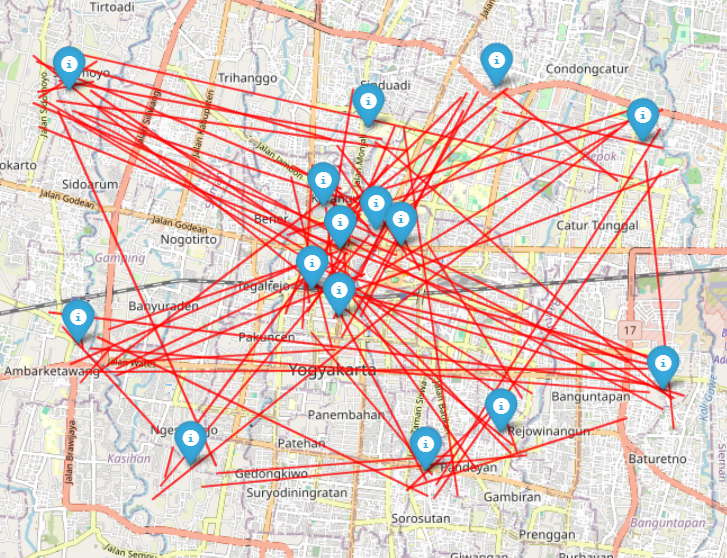
\includegraphics[scale=0.8]{Inisial.png}
    \caption{Peta Lokasi Potensial Pembangunan Stasiun}
    \label{Peta lokasi potensial pembangunan stasiun}
\end{figure}

\section{Prosedur Algoritma \textit{Fire Hawk Optimizer}}


Algoritma \textit{Fire Hawk Optimizer} (FHO) diaplikasikan untuk menyelesaikan permasalahan optimisasi lokasi stasiun pengisian daya dalam sistem \textit{electric bike-sharing}. Berikut adalah langkah-langkah utama dari algoritma FHO:

\subsection{Inisialisasi}

Langkah pertama dilakukan dengan menentukan jumlah kandidat solusi $(X)$ sebagai vektor posisi dari elang api dan mangsa. Setiap kandidat solusi merepresentasikan konfigurasi potensial dari sistem \textit{electric bike-sharing}, termasuk lokasi stasiun pengisian daya, alokasi sepeda listrik, dan trip yang diterima. Nilai awal ditentukan secara acak dalam batas-batas yang ditentukan oleh kendala sistem, seperti anggaran dan kapasitas maksimum stasiun.

\begin{align}
    X &= \begin{bmatrix}
    X_1 \\
    X_2 \\
    \vdots \\
    X_i \\
    \vdots \\
    X_N
    \end{bmatrix} 
    = \begin{bmatrix}
    x_1^1 & x_1^2 & \cdots & x_1^a & \cdots & x_1^d \\
    x_2^1 & x_2^2 & \cdots & x_2^a & \cdots & x_2^d \\
    \vdots & \vdots & & \vdots & & \vdots \\
    x_b^1 & x_b^2 & \cdots & x_b^a & \cdots & x_b^d \\
    \vdots & \vdots & & \vdots & & \vdots \\
    x_N^1 & x_N^2 & \cdots & x_N^a & \cdots & x_N^d
    \end{bmatrix},
\end{align}
dan
\begin{align}
    x_i^j(0) &= x_{i,\text{min}}^j + \text{rand}( x_{i,\text{max}}^j - x_{i,\text{min}}^j ), \quad i = 1, 2, \ldots, N, \text{ dan } j = 1, 2, \ldots, d,
\end{align}

dengan
\begin{enumerate}
    \item $X_i$ merepresentasikan kandidat solusi ke $i$ di ruang pencarian,
    \item $d$ merepresentasikan dimensi dari permasalahan (misalnya, jumlah lokasi potensial stasiun plus jumlah sepeda yang dapat dialokasikan),
    \item $N$ adalah jumlah total kandidat solusi di ruang pencarian,
    \item $x_i^j$ adalah variabel keputusan ke $j$ dari kandidat solusi ke $i$ (misalnya, keputusan untuk membangun stasiun di lokasi tertentu atau .jumlah sepeda yang dialokasikan),
    \item $x_i^j(0)$ merepresentasikan posisi awal dari kandidat solusi,
    \item $x_{i,\text{min}}^j$ dan $x_{i,\text{max}}^j$ adalah batas bawah dan batas atas dari variabel keputusan ke $j$ untuk kandidat solusi ke $i$,
    \item rand adalah bilangan acak yang terdistribusi seragam dalam rentang [0,1], dan
    \item $i = 1, 2, \ldots, N$ dan $j = 1, 2, \ldots, d$.
\end{enumerate}

\subsection{Evaluasi dan Seleksi}
Fungsi objektif ini merepresentasikan total profit yang diharapkan dari operasi sistem \textit{electric bike-sharing}, dengan mempertimbangkan pendapatan dari perjalanan yang diterima, biaya pembangunan stasiun, dan biaya operasional.\\

Beberapa kandidat solusi dengan nilai fungsi objektif terbaik direpresentasikan sebagai elang api, sedangkan kandidat solusi lain dianggap sebagai mangsa. Elang api yang dipilih dimanfaatkan untuk menyebarkan api di sekitar mangsa di ruang pencarian untuk memudahkan perburuan. Hal ini dapat diinterpretasikan sebagai eksplorasi area di sekitar solusi-solusi terbaik untuk menemukan konfigurasi sistem \textit{electric bike-sharing} yang lebih optimal.\\

Solusi terbaik global diasumsikan sebagai api utama yang pertama kali dimanfaatkan oleh elang api untuk menyebarkan api di ruang pencarian. Ini merepresentasikan konfigurasi terbaik sistem \textit{electric bike-sharing} yang ditemukan sejauh ini. Solusi-solusi yang direpresentasikan sebagai elang api dan mangsa dinyatakan dinyatakan sebagai berikut.
\begin{align}
    PR = \begin{bmatrix}
        PR_1\\
        PR_2\\
        \vdots\\
        PR_k\\
        \vdots\\
        PR_m
    \end{bmatrix},
\end{align}

dan

\begin{align}
    FH = \begin{bmatrix}
        FH_1\\
        FH_2\\
        \vdots\\
        FH_l\\
        \vdots\\
        FH_n
    \end{bmatrix},
\end{align}
dengan
\begin{enumerate}
    \item notasi $PR_k$ adalah mangsa ke-$k$ di ruang pencarian berdasarkan jumlah angka dari mangsa $m$. Mangsa-mangsa ini merepresentasikan solusi-solusi yang kurang optimal untuk sistem \textit{electric bike-sharing},
    \item notasi $FH_l$ adalah elang api ke $l$ berdasarkan jumlah dari $n$ elang api di ruang pencarian. Elang-elang api merepresentasikan solusi-solusi terbaik yang ditemukan untuk sistem \textit{electric bike-sharing},
    \item jumlah total mangsa dinotasikan $m$ (solusi kurang optimal), dan
    \item jumlah total elang api dinotasikan $n$ (solusi terbaik).
\end{enumerate}

\subsection{Penentuan Teritori}
Pada fase berikutnya, dihitung jumlah jarak antara elang api dan mangsa untuk menentukan teritori yang efektif. Jarak ini merepresentasikan perbedaan antara solusi-solusi dalam ruang pencarian sistem \textit{electric bike-sharing}. Jarak mangsa terpendek terhadap tiap elang api ditentukan, dengan mangsa terdekat dari elang api pertama memiliki fungsi objektif terbaik. Teritori dari burung lain dipertimbangkan dari rata-rata jarak mangsa yang tersisa.

\begin{align}
    D_k^l = \sqrt{(x_2-x_1)^2+(y_2-y_1)^2}, 
    \quad l = 1, 2, \ldots, n,  \text{ dan } k = 1, 2, \ldots, m,
\end{align}
dengan
\begin{enumerate}
    \item notasi $D_k^l$ adalah jumlah jarak antara elang api ke-$l$ dan mangsa ke-$m$ dalam ruang solusi sistem \textit{electric bike-sharing},
    \item jumlah mangsa di ruang pencarian dinotasikan $m$,
    \item jumlah elang api di ruang pencarian dinotasikan $n$, 
    \item Koordinat dari elang api dan mangsa di ruang pencarian direpresentasikan dengan $(x_1,y_1)$ dan $(x_2,y_2)$. Untuk sistem \textit{electric bike-sharing}, koordinat ini bisa merepresentasikan berbagai aspek konfigurasi sistem, seperti lokasi stasiun, alokasi sepeda, dan trip yang diterima, dan
    \item $l=1,2,\ldots, n$, dan $k=1,2, \ldots, m$.
\end{enumerate}

\subsection{Pembaruan Posisi Elang Api}
Elang api mengumpulkan kayu yang terbakar dari api utama untuk memantik api di area yang dipilih. Dalam algoritma optimisasi, hal ini merepresentasikan proses eksplorasi solusi baru berdasarkan solusi terbaik yang ada. Tiap burung membawa kayu yang terbakar lalu menjatuhkannya di teritori tertentu untuk memaksa mangsanya melarikan diri. Beberapa burung akan menggunakan kayu yang terbakar dari teritori elang api yang lain. Proses ini direpresentasikan dalam persamaan berikut:
\begin{align}
    FH_l^{\textit{new}}=FH_l+(r_1\times GB-r_2\times FH_{\textit{near}}), \quad l=1,2,\ldots,n,
\end{align}
dengan
\begin{enumerate}
    \item notasi $FH_l^{\textit{new}}$ adalah new vektor posisi dari elang api ($FH_l$) ke-$l$, merepresentasikan solusi baru untuk konfigurasi sistem \textit{electric bike-sharing},
    \item notasi $GB$ adalah solusi terbaik global di ruang pencarian yang dianggap sebagai api utama, merepresentasikan konfigurasi terbaik sistem yang ditemukan sejauh ini,
    \item notasi $FH_{\textit{near}}$ adalah salah satu elang api lain di ruang pencarian, merepresentasikan solusi terbaik lainnya, dan
    \item notasi $r_1$ dan $r_2$ adalah angka acak yang terdistribusi seragam dalam rentang $(0,1)$.
\end{enumerate}

\subsection{Pembaruan Posisi Mangsa}
Pergerakan mangsa di dalam teritori dari tiap elang api dianggap sebagai kunci dari perilaku hewan untuk proses pembaruan posisi. Dalam optimisasi sistem \textit{electric bike-sharing}, hal ini merepresentasikan penyesuaian solusi-solusi yang kurang optimal berdasarkan solusi-solusi terbaik yang ada. Ketika kayu yang terbakar dijatuhkan, mangsa memutuskan untuk bersembunyi, melarikan diri, atau berlari ke arah elang api secara tidak sengaja. Proses ini direpresentasikan dalam persamaan berikut:
\begin{align}
    PR_q^{\textit{new}}=PR_q+(r_3\times FH_l-r_4\times SP_l), \quad l = 1, 2, \ldots, n,  \text{ dan } q = 1, 2, \ldots, r,
\end{align}
dan
\begin{align}
    PR_q^{\textit{new}}=PR_q+(r_5\times FH_{Alter}-r_6\times SP), \quad l = 1, 2, \ldots, n,  \text{ dan } q = 1, 2, \ldots, r,
\end{align}
dengan
\begin{enumerate}
    \item notasi $PR_q^{\textit{new}}$ adalah vektor posisi baru dari mangsa ke-$q$ ($PR_q$) yang dimangsa oleh elang api ke-$l$ ($FH_l$), merepresentasikan solusi baru yang dihasilkan dari solusi yang kurang optimal,
    \item notasi $SP_l$ adalah tempat aman di dalam teritori elang api ke-$l$, merepresentasikan rata-rata dari solusi-solusi dalam teritori tertentu,
    \item notasi $SP$ adalah tempat aman di luar teritori elang api ke-$l$, merepresentasikan rata-rata global dari semua solusi,
    \item notasi $FH_{Alter}$ adalah salah satu elang api lain di ruang pencarian, merepresentasikan solusi terbaik lainnya,
    \item notasi $r_3$, $r_4$, $r_5$, $r_6$ adalah bilangan acak yang berdistribusi seragam dalam rentang $(0,1)$, dan
    \item l = 1, 2, \ldots, n,  \text{ dan } q = 1, 2, \ldots, r.
\end{enumerate}

\subsection{Tempat Aman}
Tempat aman adalah lokasi di mana sebagian besar hewan berkumpul untuk tempat berlindung dari ancaman. Dalam optimisasi, hal ini merepresentasikan area di ruang solusi yang cenderung menghasilkan solusi yang baik. $SP_l$ dan $SP$ diformulasikan sebagai berikut:
\begin{align}
    \text{SP}_1 &= \frac{\sum_{q=1}^r \text{PR}_q}{r}, \quad l = 1, 2, \ldots, n,  \text{ dan } q = 1, 2, \ldots, r,
\end{align}
dan
\begin{align}
    \text{SP} &= \frac{\sum_{k=1}^m \text{PR}_k}{m}, \quad k = 1, 2, \ldots, m,
\end{align}
dengan
\begin{enumerate}
    \item notasi $PR_q$ adalah mangsa ke-$q$ yang dikelilingi oleh elang api ke-$l$ ($FH_l$), merepresentasikan solusi yang kurang optimal dalam teritori tertentu.
    \item Notasi $PR_k$ adalah mangsa ke-$k$ di ruang pencarian, merepresentasikan semua solusi yang kurang optimal,
    \item notasi $r$ adalah jumlah mangsa dalam teritori tertentu,
    \item notasi $m$ adalah jumlah total mangsa di seluruh ruang pencarian, dan
    \item $l = 1, 2, \ldots, n$,  $q = 1, 2, \ldots, r$, dan $k = 1,2, \ldots, m$
\end{enumerate}

\subsection{Proses Iterasi dan Kriteria Penghentian}

Simulasi \textit{Fire Hawk Optimizer} terhadap formulasi yang telah dipaparkan di atas dengan hasil sebagai berikut. 
\begin{figure}[H]
    \centering
    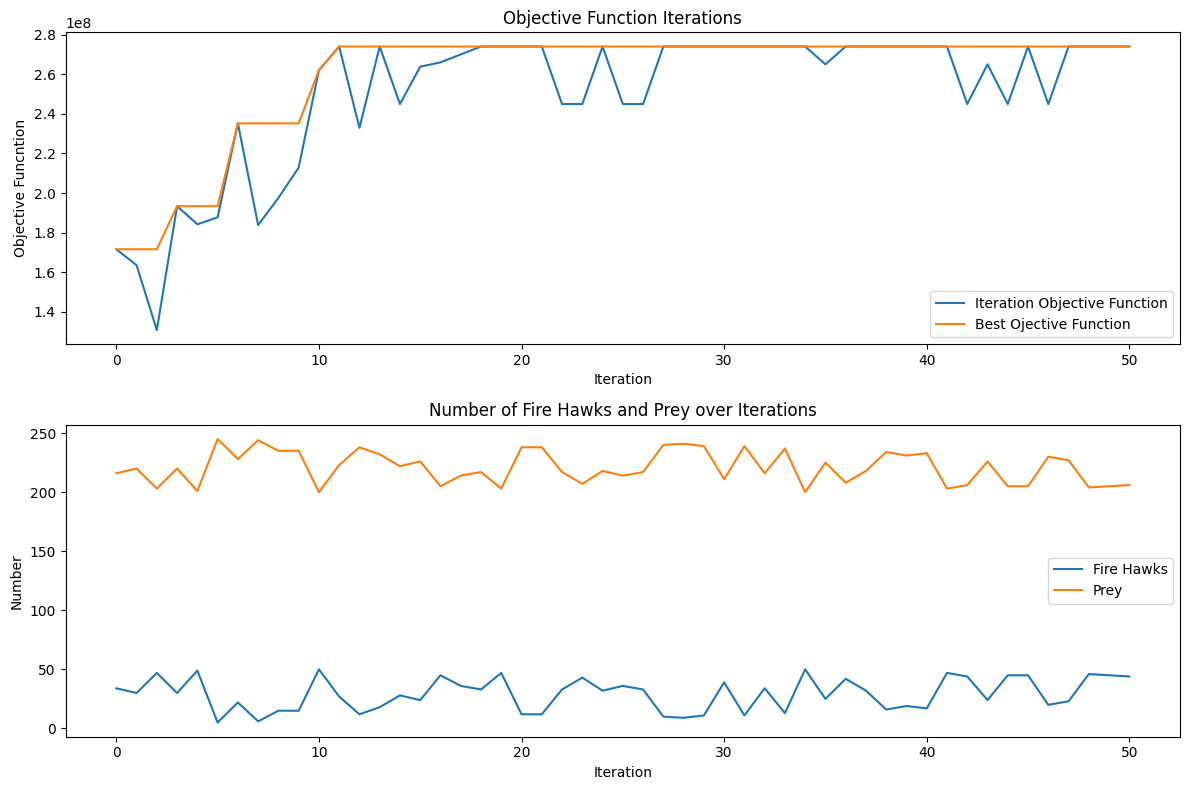
\includegraphics[scale=0.45]{__results___0_1.png}
    \caption{Iterasi Algoritma Elang Api Optimizer}
    \label{Iterasi Algoritma Fire Hawk Optimizer}
\end{figure}
Algoritma \textit{Fire Hawk Optimizer} melakukan proses iterasi untuk terus memperbaiki solusi seperti yang terlihat pada Gambar \ref{Iterasi Algoritma Fire Hawk Optimizer}. Pada setiap iterasi:
\begin{enumerate}
    \item posisi elang api dan mangsa diperbarui menggunakan persamaan yang telah didefinisikan sebelumnya,
    \item nilai fungsi objektif dari setiap solusi baru dievaluasi,
    \item solusi terbaik global ($GB$) diperbarui jika ditemukan solusi yang lebih baik, dan
    \item proses penentuan teritori, pembaruan posisi elang api, dan pembaruan posisi mangsa diulangi.
\end{enumerate}
Iterasi akan terus berlanjut hingga salah satu kriteria penghentian terpenuhi. Kriteria penghentian dapat berupa (\mycite{talbi2009metaheuristics}):
\begin{enumerate}
    \item mencapai jumlah iterasi maksimum yang telah ditentukan sebelumnya,
    \item mencapai batas waktu komputasi yang telah ditetapkan, dan
    \item mencapai tingkat konvergensi tertentu, dimana perbaikan solusi antar iterasi menjadi sangat kecil atau tidak signifikan.
\end{enumerate}
Setelah kriteria penghentian terpenuhi, algoritma akan berhenti dan mengembalikan solusi terbaik yang ditemukan sebagai konfigurasi optimal untuk sistem \textit{electric bike-sharing}. Solusi ini mencakup lokasi stasiun pengisian daya yang harus dibangun, alokasi sepeda listrik yang optimal, dan trip yang harus diterima.

\subsection{Output Simulasi}

Simulasi dilakukan dengan menggunakan \textit{Python}  dan diperoleh solusi optimal dengan menggunakan algoritma \textit{Fire Hawk Optimizer}. Gambar \ref{Peta stasiun yang dibangun dan trip yang diterima} menunjukkan lokasi stasiun yang dibuka dan trip yang diterima, dijelaskan juga hasil dari output, termasuk nilai untuk setiap variabel dan hasil fungsi objektif.

\begin{figure}[H]
    \centering
    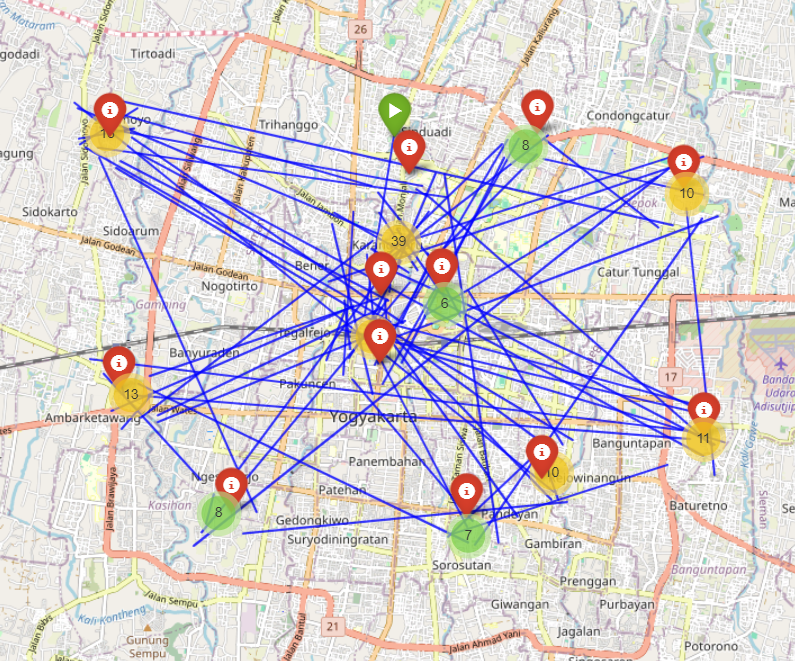
\includegraphics[scale=0.8]{hasil.png}
    \caption{Peta Stasiun yang Dibangun dan Trip yang Diterima}
    \label{Peta stasiun yang dibangun dan trip yang diterima}
\end{figure}

\subsubsection*{Variabel dan Hasil}
\begin{enumerate}
\item \textbf{Stasiun yang Dibangun ((y))}\
Solusi optimal menunjukkan bahwa dari 15 lokasi potensial, 12 stasiun dipilih untuk dibangun, yaitu stasiun [1, 2, 3, 6, 7, 8, 9, 10, 11, 12, 13, 14]. Lokasi-lokasi ini meliputi (tidak dalam urutan).
\begin{enumerate}
\item Sidomoyo,
\item Monjali,
\item Kentungan,
\item Seturan,
\item Tugu,
\item Cik di Tiro,
\item Malioboro,
\item Simpang Empat Pelem,
\item Ngastiharjo,
\item Mergangsan,
\item Rejowinangun, dan
\item Bandara Adisucipto.
\end{enumerate}
Hal ini menandakan bahwa 80\% dari lokasi potensial dianggap strategis untuk mendukung operasi sistem \textit{bike-sharing}. Pemilihan lokasi ini mencakup berbagai area penting di Yogyakarta, termasuk pusat kota, area wisata, kawasan pendidikan, area bisnis dan pemukiman, serta titik-titik transportasi penting. 
\item \textbf{Sepeda yang Dibeli (\(b\))}\\
Model merekomendasikan pembelian 55 sepeda listrik. Jumlah ini mewakili keseimbangan optimal antara memenuhi permintaan yang diperkirakan dan mengelola biaya inventaris. Berikut lokasi terakhir sepeda listrik dari seluruh skenario.\\

\begin{tabular}{llcl}\hspace{-0.3em}
    (a) & \hspace{-0.5em}Sidomoyo &: & 8 sepeda, \\
    (b) & \hspace{-0.5em}Monjali &: & 1 sepeda,\\
    (c) & \hspace{-0.5em}Ketungan &: & 2 sepeda,\\
    (d) & \hspace{-0.5em}Seturan &: & 7 sepeda,\\
    (e) & \hspace{-0.5em}Tugu &: & 4  sepeda,\\
    (f) & \hspace{-0.5em}Cik di Tiro &: & 5 sepeda,\\
    (g) & \hspace{-0.5em}Malioboro &: & 7 sepeda,\\
    (h) & \hspace{-0.5em}Simpang Empat Pelem &: & 5 sepeda,\\
    (i) & \hspace{-0.5em}Ngastiharjo &: & 3 sepeda,\\
    (j) & \hspace{-0.5em}Mergangsan &: & 8 sepeda,\\
    (k) & \hspace{-0.5em}Rejowinangun &: & 7 sepeda, dan\\
    (l) & \hspace{-0.5em}Bandara Adisucipto &: & 4 sepeda.\\
\end{tabular}
\item \textbf{Trip yang Diterima (\(x\))}\\
Tingkat penerimaan trip bervariasi di antara skenario:
\begin{enumerate}
    \item Skenario 0 (Weekdays): 25/30 trip diterima (83.33\%)
    \item Skenario 1 (Saturday): 28/30 trip diterima (93.33\%)
    \item Skenario 2 (Sunday): 27/30 trip diterima (90.00\%)
\end{enumerate}
Tingkat penerimaan yang tinggi ini menunjukkan bahwa sistem yang diusulkan mampu memenuhi sebagian besar permintaan yang diproyeksikan, dengan kinerja terbaik pada hari Sabtu.
\end{enumerate}

Secara keseluruhan, solusi ini menunjukkan desain sistem \textit{bike-sharing} yang efisien terhadap permintaan dengan potensi keuntungan yang signifikan. Namun, masih ada ruang untuk penyempurnaan lebih lanjut, terutama dalam hal peningkatan utilisasi sepeda dan posibilitas optimasi lebih lanjut dari lokasi stasiun.